% Hiring and Firing -- the backtesting ideas applied to the market for managers.
% Figures and every number quoted here come from hiring_and_firing_figures.py
\documentclass[aspectratio=169,10pt]{beamer}
\usetheme{default}
\usecolortheme{default}

\usepackage{graphicx}
\usepackage{adjustbox}
\usepackage{amsmath}
\usepackage{amssymb}
\usepackage{booktabs}
\usepackage{tikz}
\usetikzlibrary{arrows.meta,positioning,calc,shadows}
\usepackage{appendixnumberbeamer}  % Exclude appendix from slide count

\setbeamertemplate{navigation symbols}{}
\setbeamertemplate{items}[circle]

% Footline: Author, Event (Year) on left; page/total on right
\setbeamertemplate{footline}{
  \hbox{%
    \begin{beamercolorbox}[wd=.5\paperwidth,ht=2.5ex,dp=1ex,left]{author in head/foot}%
      \hspace*{2ex}\insertshortauthor, \insertshortinstitute\ (\insertdate)
    \end{beamercolorbox}%
    \begin{beamercolorbox}[wd=.5\paperwidth,ht=2.5ex,dp=1ex,right]{date in head/foot}%
      \insertframenumber/\inserttotalframenumber\hspace*{2ex}
    \end{beamercolorbox}%
  }
}

% Highlight boxes
\setbeamercolor{box1}{bg=red!12,fg=black}

% A press clipping: [rotation]{outlet}{date}{width}{headline, paraphrased}
\newcommand{\newscard}[5][0]{%
  \tikz\node[rotate=#1, draw=black!18, fill=white, rounded corners=2pt, drop shadow={opacity=0.22},
             inner sep=7pt, text width=#4, align=left]{%
    {\scriptsize\bfseries\textcolor{black!75}{#2}\hfill\textcolor{black!50}{#3}}\\[-2pt]
    {\color{black!15}\rule{\linewidth}{0.4pt}}\\[0pt]
    {\small #5}};}
% A poll option: {colour}{letter and choice}
\newcommand{\pollbox}[2]{\tikz\node[draw=#1!65!black, fill=#1!10, rounded corners=4pt, minimum width=3.7cm,
                                   minimum height=1.1cm, align=center, font=\large]{#2};}
\newcommand{\bignum}[1]{{\fontsize{44}{48}\selectfont\textbf{\textcolor{red!75!black}{#1}}}}

\title{Hiring and Firing}
\subtitle{Strategies, managers, and one decision problem}
\author[A. Moreira]{Alan Moreira}
\institute[Data-Driven Investing]{NYU Stern --- Data-Driven Investing}
\date{Fall 2026}

\begin{document}

%------------------------------------------------------------------ 1
\begin{frame}
\titlepage
\end{frame}

%------------------------------------------------------------------ M1  (Melvin opening: the fund is anonymous until M4)
\begin{frame}{Would you invest with this manager?}
\begin{columns}[c]
\begin{column}{0.60\textwidth}
\adjustbox{max width=\textwidth}{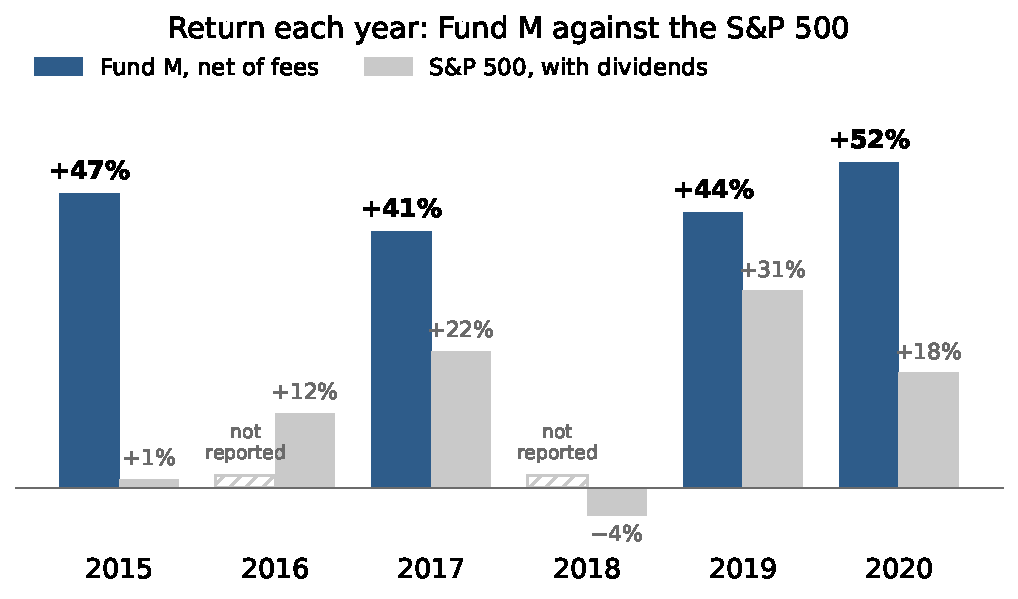
\includegraphics{figures/melvin_record.pdf}}
\end{column}
\begin{column}{0.38\textwidth}
\begin{itemize}
\item About \textcolor{red}{30\% a year}, 2014--2020
\vskip 8pt
\item The S\&P 500 over 2015--2020: about 13\% a year
\vskip 8pt
\item $+52\%$ in 2020
\vskip 8pt
\item \$12.5 billion to manage by January 2021
\vskip 8pt
\item Long-short US equity, run by a star stock-picker
\end{itemize}
\end{column}
\end{columns}
\end{frame}

%------------------------------------------------------------------ M2
\begin{frame}{January 2021: you are an investor. What do you do?}
\begin{columns}[c]
\begin{column}{0.60\textwidth}
\adjustbox{max width=\textwidth}{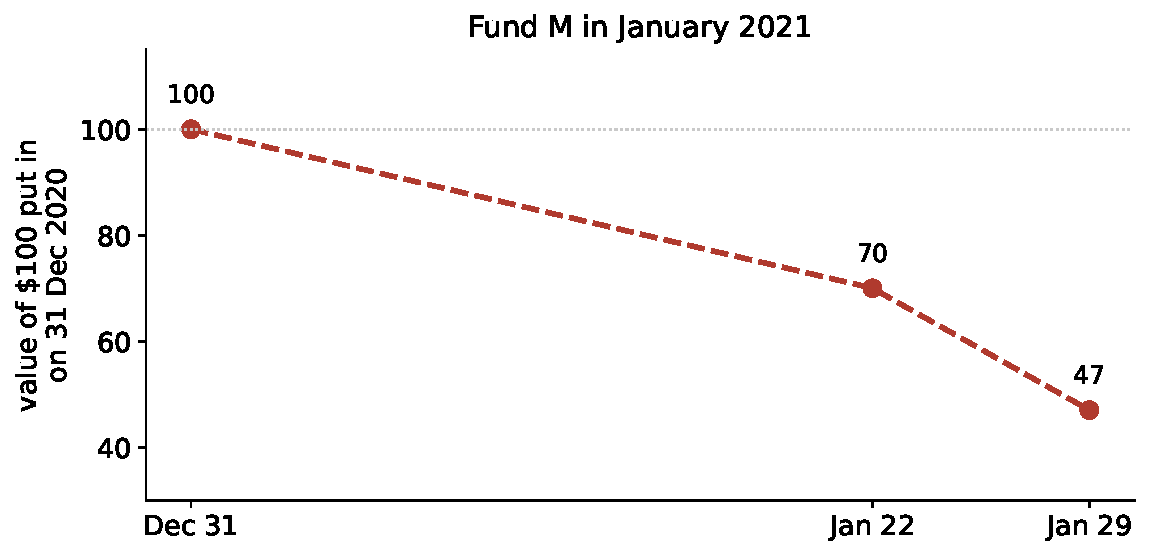
\includegraphics{figures/melvin_january.pdf}}
\end{column}
\begin{column}{0.38\textwidth}
\centering
\bignum{$-53\%$}\\[2pt]
in one month
\end{column}
\end{columns}
\vskip 10pt
\begin{center}
\pollbox{red}{\textbf{A}\ \ Take your money out} \hfill
\pollbox{gray}{\textbf{B}\ \ Stay} \hfill
\pollbox{blue}{\textbf{C}\ \ Put more in}
\end{center}
\end{frame}

%------------------------------------------------------------------ M3
\begin{frame}{Two of the best-informed investors in the business chose C}
\vskip 4pt
\begin{center}
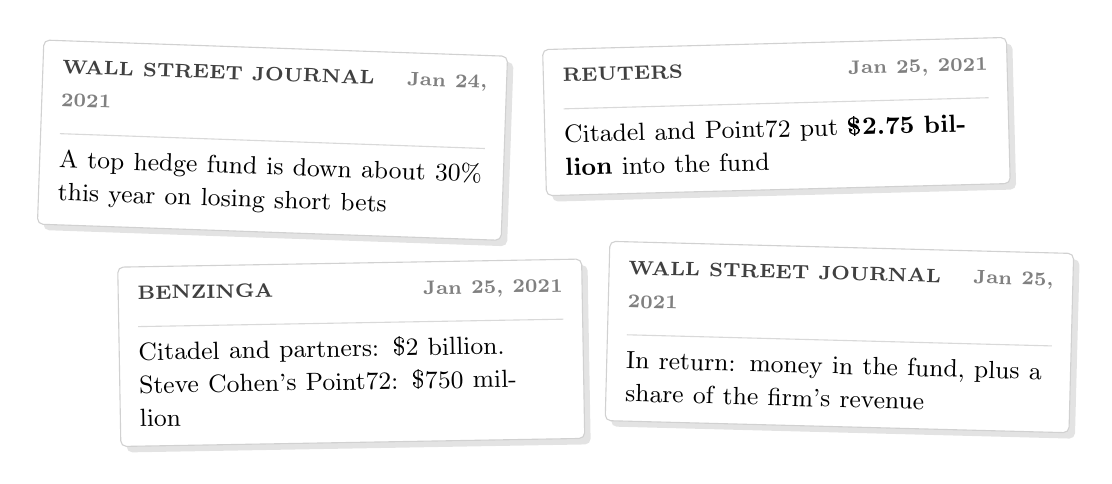
\begin{tikzpicture}
\node at (0, 1.2)   {\newscard[-2]{WALL STREET JOURNAL}{Jan 24, 2021}{5.4cm}{A top hedge fund is down about 30\% this year on losing short bets}};
\node at (6.4, 1.5) {\newscard[1.5]{REUTERS}{Jan 25, 2021}{5.4cm}{Citadel and Point72 put \textbf{\$2.75 billion} into the fund}};
\node at (1.0, -1.5){\newscard[1]{BENZINGA}{Jan 25, 2021}{5.4cm}{Citadel and partners: \$2 billion. Steve Cohen's Point72: \$750 million}};
\node at (7.2, -1.3){\newscard[-1.5]{WALL STREET JOURNAL}{Jan 25, 2021}{5.4cm}{In return: money in the fund, plus a share of the firm's revenue}};
\end{tikzpicture}
\end{center}
\vskip 4pt
\begin{center}
They put money in during the worst week. \textcolor{red}{Why?}
\end{center}
\end{frame}

%------------------------------------------------------------------ M4
\begin{frame}{Fund M is Melvin Capital, and the trade was GameStop}
\begin{columns}[c]
\begin{column}{0.42\textwidth}
\begin{itemize}
\item Founded in 2014 by Gabe Plotkin, one of Steve Cohen's top portfolio managers at SAC Capital
\vskip 7pt
\item Melvin was short GameStop
\vskip 7pt
\item Retail traders on Reddit's r/wallstreetbets bid the stock up \textcolor{red}{18-fold} in four weeks
\vskip 7pt
\item Jan 28: Robinhood restricts buying of GameStop
\end{itemize}
\end{column}
\begin{column}{0.56\textwidth}
\adjustbox{max width=\textwidth}{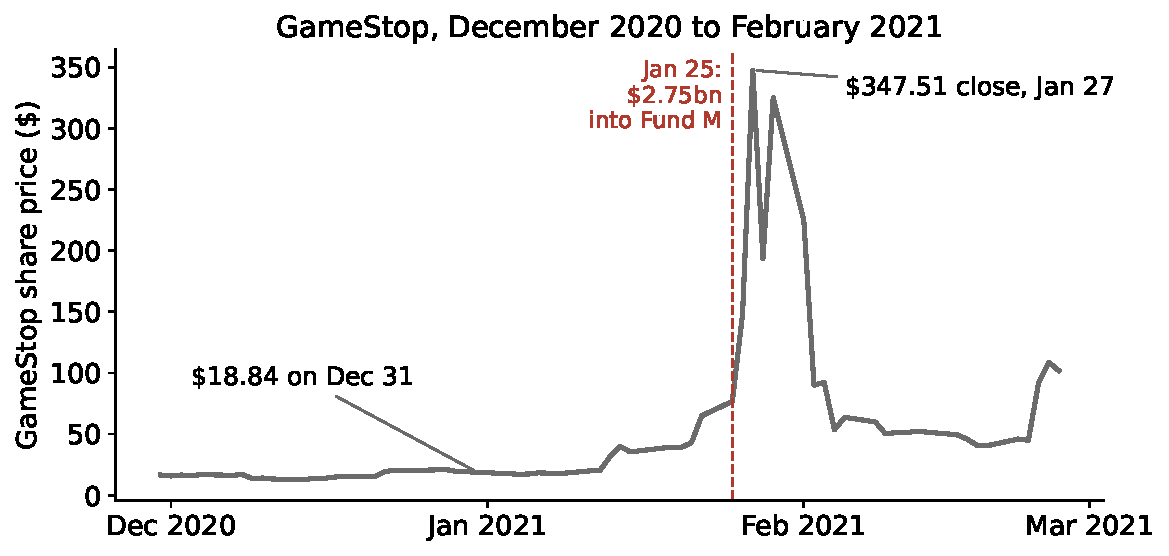
\includegraphics{figures/gme_squeeze.pdf}}
\vskip 4pt
\hfill\newscard[-1]{REUTERS}{Feb 1, 2021}{5.6cm}{Melvin lost 53\% in January. It ends the month with about \$8 billion, new money included}
\end{column}
\end{columns}
\end{frame}

%------------------------------------------------------------------ M5
\begin{frame}{What did Citadel and Point72 know that you did not?}
\begin{itemize}
\item Cohen had watched Plotkin's process up close for years at SAC
\vskip 10pt
\item Point72 already had money in Melvin before January
\vskip 10pt
\item To them, the loss looked like one crowded short squeezed by retail buying, not a failed process
\vskip 10pt
\item They also bought a share of Melvin's revenue: a stake in the business, not only in the fund
\end{itemize}
\vskip 10pt
\begin{center}
\textbf{If you trust the manager, January says little about his skill, and it may be a good time to get in}
\end{center}
\end{frame}

%------------------------------------------------------------------ M6
\begin{frame}[label=melvinodds]{Same month, two readings}
Suppose a month like January is \textbf{three times} likelier from an unskilled manager than from a skilled one.
\vskip 6pt
\begin{center}
\renewcommand{\arraystretch}{1.5}
\begin{tabular}{lccc}
\toprule
 & \multicolumn{2}{c}{odds that he is skilled} & \\
\cmidrule(lr){2-3}
 & before January & after January & what you do \\
\midrule
Citadel, Point72 & 9 to 1 \ (90\%) & 3 to 1 \ (\textcolor{red}{75\%}) & put money in \\
an investor with no inside view & 1 to 1 \ (50\%) & 1 to 3 \ (\textcolor{red}{25\%}) & take money out \\
\bottomrule
\end{tabular}
\end{center}
\vskip 6pt
\begin{itemize}
\item The same news divides both odds by three. Where you end up depends on where you started.
\hfill \hyperlink{bayes}{\beamerbutton{The formal version}}
\end{itemize}
\end{frame}

%------------------------------------------------------------------ M7
\begin{frame}{What happened next}
\begin{center}
\adjustbox{max width=0.86\textwidth, max height=0.56\textheight}{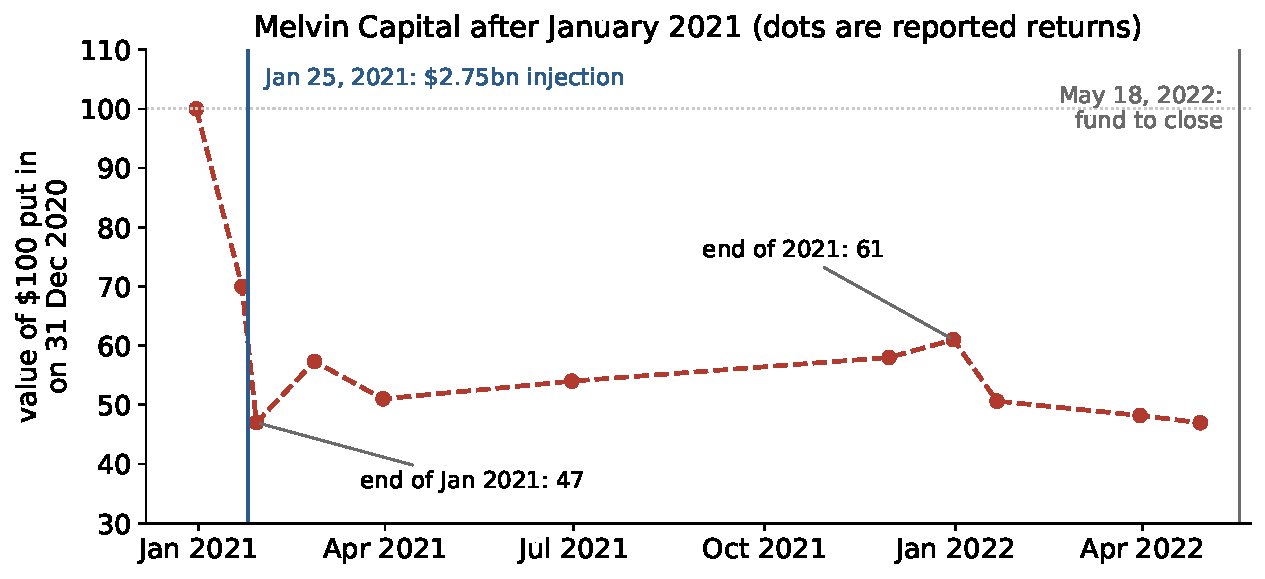
\includegraphics{figures/melvin_after.pdf}}
\end{center}
\vskip -2pt
\begin{itemize}
\item Money put in at the end of January gained about \textcolor{red}{30\%} over the rest of 2021. Money already in lost 39\% for the year.
\vskip 4pt
\item Citadel and Point72 took their money out in 2021--22. Melvin closed in May 2022.
\hfill \hyperlink{melvinsources}{\beamerbutton{Sources}}
\end{itemize}
\end{frame}

%------------------------------------------------------------------ M8
\begin{frame}{The question behind every hire and every fire}
\begin{itemize}
\item Going in and getting out are statistical decisions
\vskip 10pt
\item How far bad news moves you depends on what you knew before it arrived
\vskip 10pt
\item One outcome does not grade the decision: Melvin closed, yet money that came in after the January crash gained about 30\% over the rest of 2021
\end{itemize}
\vskip 16pt
\begin{beamercolorbox}[rounded=true,sep=8pt,center]{box1}
Same returns, different priors, opposite decisions
\end{beamercolorbox}
\end{frame}

%------------------------------------------------------------------ 2
\begin{frame}{Going into a strategy is a statistical decision}
You never see the true appraisal ratio. You see an estimate, from $T$ years of data. Only unbiased data counts (Test--not EST/TUNE!)
\vskip 10pt
\[ \text{go in when} \qquad \widehat{AR}_T \;\ge\; a^{*} + \frac{z_p}{\sqrt{T}} \]
\vskip 6pt
\begin{itemize}
\item $a^{*}$: your hurdle
\vskip 8pt
\item $z_p$: how sure you need to be (1.64 for 95\%)
\vskip 8pt
\item $1/\sqrt{T}$: the standard error of the estimate

\item This decision rule implies 95\% of the strategies you got into will have appraisal higher than the hurdle
\end{itemize}
\end{frame}

%------------------------------------------------------------------ 3
\begin{frame}{Walking away is the mirror image}
Give up once you are sure enough that the strategy does \emph{not} meet your goal.
\vskip 10pt
\[ \text{walk away when} \qquad \widehat{AR}_T \;\le\; a^{*} - \frac{z_p}{\sqrt{T}} \]
\vskip 14pt
\begin{beamercolorbox}[rounded=true,sep=8pt,center]{box1}
The same three ingredients: a \textbf{goal}, a \textbf{confidence}, and \textbf{time}
\end{beamercolorbox}
\vskip 10pt
\begin{itemize}
\item In between the two lines, you do not know yet
\end{itemize}
\end{frame}

%------------------------------------------------------------------ 4
\begin{frame}{The walk-away line}
\begin{center}
\adjustbox{max width=\textwidth, max height=0.66\textheight}{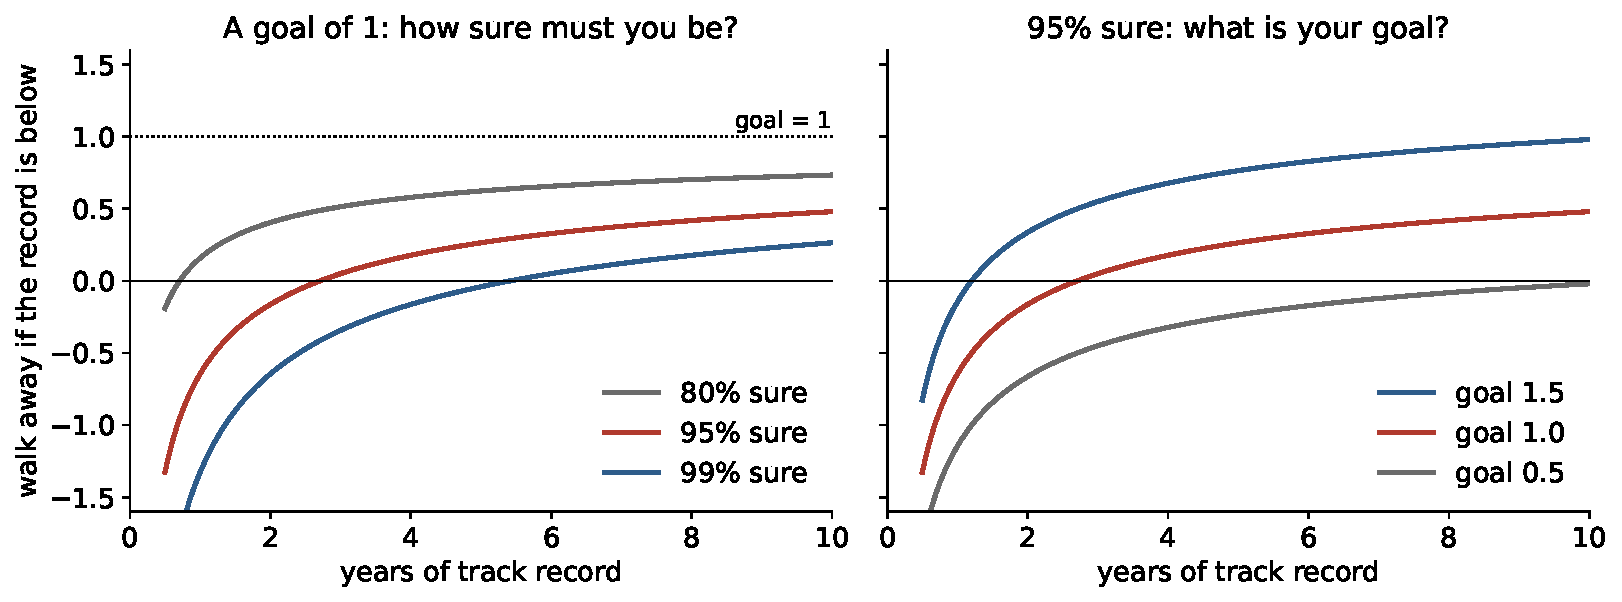
\includegraphics{figures/walk_away.pdf}}
\end{center}
\vskip 2pt
\begin{itemize}
\item More confidence means more patience. A higher goal lifts the whole line.
\end{itemize}
\end{frame}

%------------------------------------------------------------------ 5
\begin{frame}{Three levers}
Your goal is an appraisal ratio of 1. Walk away if the record is below:
\vskip 4pt
\begin{center}
\renewcommand{\arraystretch}{1.3}
\begin{tabular}{cccc}
\toprule
years of record & 80\% sure & 95\% sure & 99\% sure \\
\midrule
1 & 0.16 & \textcolor{red}{$-$0.64} & $-$1.33 \\
3 & 0.51 & 0.05 & $-$0.34 \\
5 & 0.62 & 0.26 & $-$0.04 \\
10 & 0.73 & 0.48 & 0.26 \\
\bottomrule
\end{tabular}
\end{center}
\vskip 6pt
\begin{itemize}
\item After one year, only a record below $-0.64$ sends you away at 95\%
\vskip 6pt
\item Time is the only lever that brings the line up to the goal
\end{itemize}
\end{frame}

%------------------------------------------------------------------ 6
\begin{frame}{A manager is a strategy you cannot backtest}
\begin{itemize}
\item Hiring is going in. Firing is walking away.
\vskip 14pt
\item The same three ingredients apply: a goal, a confidence, and time
\vskip 14pt
\item What is different: before you hire, you often have \textcolor{red}{no returns at all}, only what your selection process tells you
\end{itemize}
\end{frame}

%------------------------------------------------------------------ 14
\begin{frame}{With a track record, the strategy logic applies}
\[ t \;=\; \widehat{AR}_T \times \sqrt{T} \]
\vskip 4pt
\begin{itemize}
\item Three years at an appraisal ratio of 1: $t = 1.7$
\vskip 10pt
\item Ten years at 0.5: $t = 1.6$
\vskip 10pt
\item The record moves your belief before you have a single day of your own evidence
\end{itemize}
\end{frame}

%------------------------------------------------------------------ 15
\begin{frame}{But the record you are shown was selected}
\begin{itemize}
\item Of 100 managers with no skill, 5 will have a record that clears the 95\% bar
\vskip 12pt
\item Those are the ones who come to see you
\end{itemize}
\vskip 16pt
\begin{beamercolorbox}[rounded=true,sep=8pt,center]{box1}
Their record is the \textbf{estimate} sample. The \textbf{test} starts the day you hire.
\end{beamercolorbox}
\end{frame}

%================================================================== THE NOTEBOOK
\begin{frame}{Now: the notebook}
\vskip 2pt
\begin{beamercolorbox}[rounded=true,sep=7pt,center]{box1}
\textbf{Notebook: Hiring and Firing} \ --- \ would you have hired Warren Buffett? And fired him?
\end{beamercolorbox}
\vskip 10pt
\begin{enumerate}
\item \textbf{Would you hire him?} Slide through his record, 1989--1998, against the hire line.
\vskip 5pt
\item \textbf{The test starts the day you hire.} You hire him in January 1999. Slide his record since then against the walk-away line.
\vskip 5pt
\item \textbf{What happened next.} What firing him cost you.
\end{enumerate}
\vskip 8pt
{\small \textbf{Bring back:} the rule only saw his returns. What did it not know? \\[2pt]
Stop at \textbf{Back to the slides}; the challenge after it is homework.}
\end{frame}
%================================================================== BACK TO THE SLIDES
%------------------------------------------------------------------ 7
\begin{frame}{The hiring process}
\begin{center}
\adjustbox{max width=\textwidth}{%
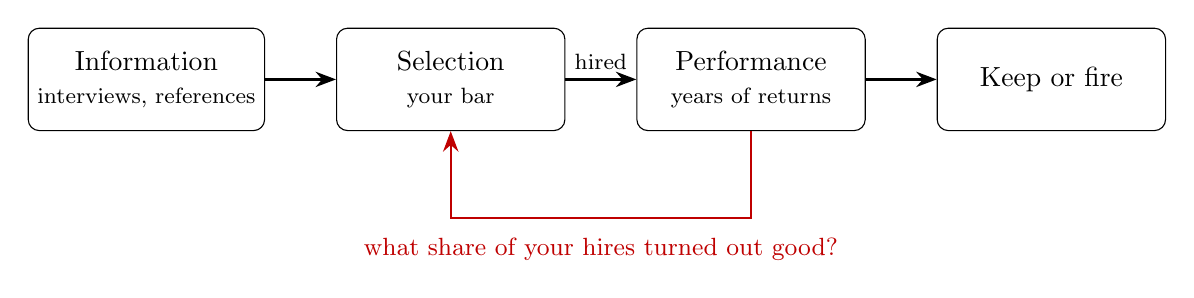
\begin{tikzpicture}[node distance=9mm,
  box/.style={draw, rounded corners, minimum height=13mm, minimum width=29mm, align=center},
  arr/.style={-{Stealth[length=2.6mm]}, thick}]
\node[box] (info) {Information\\ {\footnotesize interviews, references}};
\node[box, right=of info] (sel) {Selection\\ {\footnotesize your bar}};
\node[box, right=of sel] (perf) {Performance\\ {\footnotesize years of returns}};
\node[box, right=of perf] (dec) {Keep or fire};
\draw[arr] (info) -- (sel);
\draw[arr] (sel) -- node[above, font=\footnotesize]{hired} (perf);
\draw[arr] (perf) -- (dec);
\draw[arr, red!75!black] (perf.south) -- ++(0,-11mm) -| (sel.south);
\node[font=\small, red!75!black] at ($(sel.south)!0.5!(perf.south) + (0,-15mm)$) {what share of your hires turned out good?};
\end{tikzpicture}}
\end{center}
\vskip 10pt
\begin{itemize}
\item The walk-away rule sees only the third box. It does not know how the manager got there.
\vskip 8pt
\item Performance grades the manager, and it grades your process
\end{itemize}
\end{frame}

%------------------------------------------------------------------ 8
\begin{frame}{No track record: you are betting on your process}
\begin{itemize}
\item With no returns to look at, your belief that a hire is good is your \textcolor{red}{hit rate}
\vskip 14pt
\item The share of the people your process lets in who turn out good
\vskip 14pt
\item Returns then move that belief, one year at a time
\end{itemize}
\end{frame}

%------------------------------------------------------------------ 9
\begin{frame}{The same bad years, two readings}
\begin{itemize}
\item \textbf{Strong process}: most of your hires are good, so a bad stretch is probably bad luck
\vskip 14pt
\item \textbf{Weak process}: few of your hires are good, so a bad stretch is probably the truth
\vskip 14pt
\item The returns are the same. What differs is what you believed before you saw them.
\vskip 14pt
\item Melvin, January 2021: Citadel and Point72 read it the first way
\end{itemize}
\end{frame}

%------------------------------------------------------------------ 9b  (was appendix A1 + A4)
\begin{frame}[label=bayes]{How much two flat years should move you}
Two kinds of manager: good (appraisal ratio $a$) or unskilled (zero). A $T$-year record is the truth plus noise, standard error $1/\sqrt{T}$.
\[ \underbrace{\frac{\pi_T}{1-\pi_T}}_{\text{odds after the record}} \;=\;
   \underbrace{\frac{\pi}{1-\pi}}_{\text{odds at hire}} \;\times\;
   \underbrace{\exp\!\big( T\,a\,(\widehat{AR}_T - a/2) \big)}_{\text{how much likelier the record is if good}} \]
Hired to deliver $a = 1$, two years at zero: \ $\exp\!\big(2 \times 1 \times (0 - 0.5)\big) = \textcolor{red}{0.37}$
\vskip 2pt
\begin{center}
\renewcommand{\arraystretch}{1.2}
\begin{tabular}{cccc}
\toprule
share of your hires who are good & odds at hire & odds after ($\times\,0.37$) & chance still good \\
\midrule
80\% & 4.00 & 1.47 & \textcolor{red}{60\%} \\
50\% & 1.00 & 0.37 & 27\% \\
20\% & 0.25 & 0.09 & \textcolor{red}{8\%} \\
\bottomrule
\end{tabular}
\end{center}
\end{frame}

%------------------------------------------------------------------ 10
\begin{frame}[label=fire]{How sure you must be to fire depends on your process}
\begin{itemize}
\item Trust your process: demand \textcolor{red}{more} confidence before you fire
\vskip 12pt
\item Doubt your process: fire on \textcolor{red}{less}
\vskip 12pt
\item Two years in, hired to deliver 1: a strong process (80\% good) fires only when \textcolor{red}{95\%} sure, a coin flip at 76\%, a weak one (20\%) at 39\%
\end{itemize}
\vskip 14pt
\begin{beamercolorbox}[rounded=true,sep=8pt,center]{box1}
Firing means the returns have overturned what your process told you
\end{beamercolorbox}
\vskip 10pt
\hfill \hyperlink{appendix_fire}{\beamerbutton{The fire rule}}
\end{frame}

%------------------------------------------------------------------ 11
\begin{frame}[label=costs]{What a hire costs, and what it pays}
Your book has a Sharpe ratio of 0.5. You give the manager the risk their promise deserves.
\vskip 4pt
\begin{center}
\renewcommand{\arraystretch}{1.5}
\begin{tabular}{ccc}
\toprule
hired to deliver & your Sharpe ratio if they are good & if they have no skill \\
\midrule
1.0 & 1.12 \;($+$0.62) & \textcolor{red}{0.22 \;($-$0.28)} \\
0.5 & 0.71 \;($+$0.21) & 0.35 \;($-$0.15) \\
\bottomrule
\end{tabular}
\end{center}
\vskip 8pt
\begin{itemize}
\item A manager with no skill adds risk and nothing else
\hfill \hyperlink{appendix_sharpe}{\beamerbutton{Details}}
\end{itemize}
\end{frame}

%------------------------------------------------------------------ 12
\begin{frame}{How long each one lasts}
\[ \text{hire if} \qquad \underbrace{\pi \times \text{gain} \times \text{years the edge lasts}}_{\text{a good one}}
   \;>\; \underbrace{(1-\pi) \times \text{loss} \times \text{years until you fire}}_{\text{a bad one}} \]
\vskip 2pt
\begin{center}
\renewcommand{\arraystretch}{1.4}
\begin{tabular}{cccc}
\toprule
hired to deliver & gain, lasting & loss, lasting & break-even share good \\
\midrule
1.0 & $+$0.62, 5 years & $-$0.28, 2.7 years & \textcolor{red}{19\%} \\
0.5 & $+$0.21, 5 years & $-$0.15, 10.8 years & 60\% \\
\bottomrule
\end{tabular}
\end{center}
\vskip 6pt
\begin{itemize}
\item Skill you can detect fast: one good hire in five is enough. Slow to detect: you need three in five.
\end{itemize}
\end{frame}

%------------------------------------------------------------------ 13
\begin{frame}[label=calibrate]{Calibrating the bar}
\begin{itemize}
\item \textbf{Nearly all your hires are good?} Your bar is too high. You are leaving talent out, and you can always fire the bad ones.
\vskip 14pt
\item \textbf{Fewer good than the break-even share?} Tighten the bar
\vskip 14pt
\item Your hit rate is an estimate too. Ten hires from a process that is right half the time can easily show \textcolor{red}{3 good ones, or 7}
\end{itemize}
\end{frame}

%------------------------------------------------------------------ 13b  (was appendix A2 + A3)
\begin{frame}{How do you know your hit rate?}
You never see who is good, only records. Averaged over your past hires, the noise washes out:
\[ \hat{\pi} \;=\; \frac{\text{average record of your past hires}}{a}
   \qquad\qquad
   SE(\hat{\pi}) \;=\; \frac{1}{\sqrt{N}}\,\sqrt{\pi(1-\pi) + \frac{1}{a^{2}\,T}} \]
\begin{center}
\renewcommand{\arraystretch}{1.2}
\begin{tabular}{lccc}
\toprule
 & \multicolumn{3}{c}{years of record per hire} \\
\cmidrule(lr){2-4}
standard error of $\hat{\pi}$ \ (when $\hat{\pi} = 0.6$, $a = 1$) & 1 & 2 & 5 \\
\midrule
10 hires & 0.35 & 0.27 & 0.21 \\
20 hires & 0.25 & \textcolor{red}{0.19} & 0.15 \\
50 hires & 0.16 & 0.12 & 0.09 \\
\bottomrule
\end{tabular}
\end{center}
\begin{itemize}
\item Longer records shrink only the $1/(a^{2}T)$ term; more hires shrink both. Grade every hire over the same window, the fired ones included.
\end{itemize}
\end{frame}

%------------------------------------------------------------------ 16
\begin{frame}{One decision problem}
\begin{center}
\renewcommand{\arraystretch}{1.6}
\begin{tabular}{lll}
\toprule
 & a strategy & a manager \\
\midrule
going in & record above $a^{*} + z_p/\sqrt{T}$ & your process, plus any record \\
walking away & record below $a^{*} - z_p/\sqrt{T}$ & the same test \\
your patience & confidence in the idea & confidence in your process \\
\bottomrule
\end{tabular}
\end{center}
\vskip 10pt
\begin{itemize}
\item Every exit is also evidence about how you entered
\end{itemize}
\vskip 14pt
{\small \textbf{Homework:} the challenge at the end of the notebook. The Buffett call again, this time with a prior.}
\end{frame}

%================================================================== appendix
\appendix
\begin{frame}
\begin{center}
{\Large Appendix}
\end{center}
\end{frame}

\begin{frame}[label=appendix_fire]{A1: When to fire}
Fire once the manager is more likely unskilled than good: the odds after the record fall below 1.
\[ \widehat{AR}_T \;<\; \frac{a}{2} \;-\; \frac{1}{a\,T}\,\ln\frac{\pi}{1-\pi} \]
\vskip -6pt
\begin{center}
\adjustbox{max width=0.8\textwidth, max height=0.52\textheight}{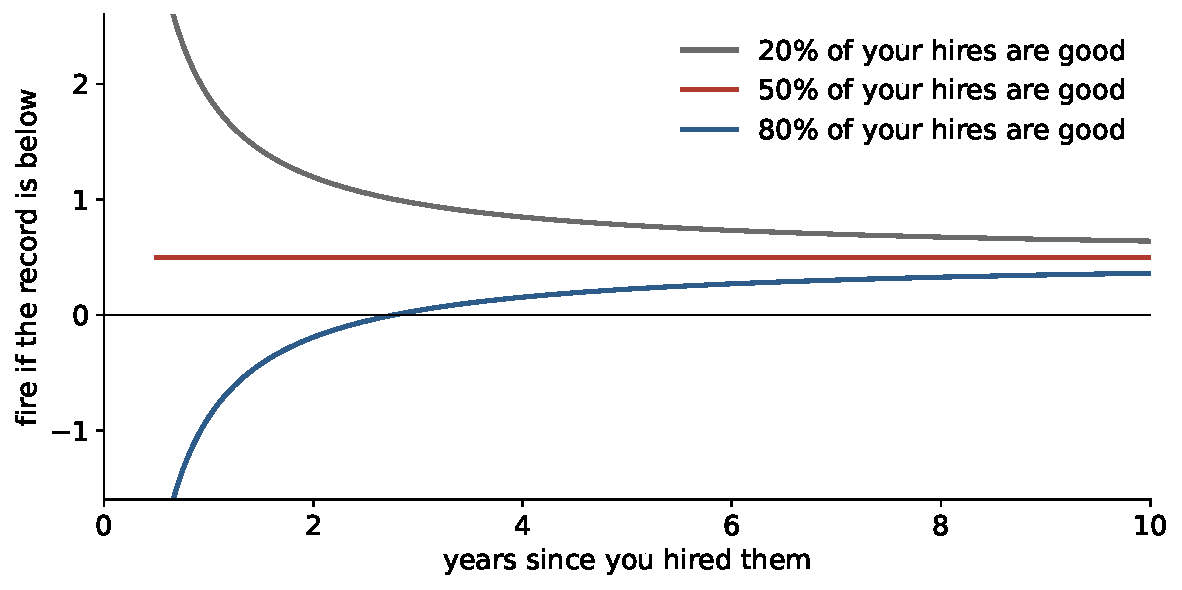
\includegraphics{figures/fire_by_process.pdf}}
\end{center}
\vskip -4pt
\hfill \hyperlink{fire}{\beamerreturnbutton{Back}}
\end{frame}

\begin{frame}{A2: The same rule, as a confidence level}
Hired to deliver 1, two years in. When the record hits the fire line, how sure are you that the manager is below the goal?
\vskip 4pt
\begin{center}
\renewcommand{\arraystretch}{1.4}
\begin{tabular}{ccc}
\toprule
share of your hires who are good & fire if the record is below & how sure you are by then \\
\midrule
80\% & $-$0.19 & \textcolor{red}{95\%} \\
50\% & 0.50 & 76\% \\
20\% & 1.19 & 39\% \\
\bottomrule
\end{tabular}
\end{center}
\vskip 4pt
\begin{itemize}
\item How sure: $\Phi\big( (a - \text{line}) \times \sqrt{T} \big)$, the walk-away calculation run in reverse
\vskip 5pt
\item A stronger process sets a lower line, so you fire only at higher confidence
\end{itemize}
\hfill \hyperlink{fire}{\beamerreturnbutton{Back}}
\end{frame}

\begin{frame}[label=appendix_sharpe]{A3: The Sharpe ratio arithmetic}
\begin{itemize}
\item Your book alone has Sharpe ratio $S$. The manager is hired to deliver appraisal ratio $a$, uncorrelated with your book.
\vskip 10pt
\item The best mix gives the manager risk in proportion $a / S$ to your book's
\vskip 10pt
\item \textbf{If they are good}: \quad $\sqrt{S^2 + a^2}$
\vskip 10pt
\item \textbf{If they have no skill}: same risk, no extra return: \quad $S^2 \big/ \sqrt{S^2 + a^2}$
\vskip 10pt
\item \textbf{Years until you fire}: $(1.64 / a)^2$, to be 95\% sure they are below the goal
\end{itemize}
\vskip 4pt
\hfill \hyperlink{costs}{\beamerreturnbutton{Back}}
\end{frame}

\begin{frame}[label=melvinsources]{A4: Sources for the Melvin example}
\footnotesize
\begin{itemize}
\item \textbf{Annual and 2021 returns}, as reported in the press and compiled in Wikipedia, ``Melvin Capital'': 2015 $+47\%$, 2017 $+41\%$, 2019 $+44\%$, 2020 $+52\%$ (2016 and 2018 not reported; about 30\% a year 2014--2020). January 2021 $-53\%$, February $+22\%$, year to date $-49\%$ (March), $-46\%$ (June), $-42\%$ (November), $-39\%$ for 2021.
\item \textbf{The injection.} WSJ, 24--25 Jan 2021: down about 30\% so far in 2021; \$2.75bn from Citadel and Point72 for money in the fund and non-controlling revenue shares. Benzinga, 25 Jan 2021: \$2bn from Citadel and partners, \$750m from Point72.
\item \textbf{End of January.} Reuters, 1 Feb 2021: $-53\%$ in January; about \$12.5bn at the start of the year, over \$8bn at the end of January with the new money.
\item \textbf{2022.} Reuters: $-17\%$ in the first three weeks of January 2022, $-23\%$ through April. CNBC: $-21\%$ in the first quarter.
\item \textbf{Exits.} Bloomberg, 24 Feb 2022: Citadel pulling back most of its \$2bn. Bloomberg, 12 Mar 2022: Point72 to redeem its \$750m (a separate Point72 stake stayed). Melvin's letter, 18 May 2022: the funds will close.
\item \textbf{GameStop prices}: Yahoo Finance, multiplied by 4 to undo the July 2022 split, so they match the prices traded in 2021. \textbf{S\&P 500}: total return index (\texttt{\^{}SP500TR}), Yahoo Finance, year end to year end.
\item Between reported dates the fund's path is not known; the chart joins the reported points with dashed lines.
\end{itemize}
\hfill \hyperlink{melvinodds}{\beamerreturnbutton{Back}}
\end{frame}

\end{document}
